\documentclass[../main/main.tex]{subfiles}
\graphicspath{{./figures/}}

\makeatletter
\renewcommand{\@chapapp}{Travaux pratiques -- TP}
\makeatother

\toggletrue{student}
\HideSolutionstrue
\toggletrue{corrige}
% \renewcommand{\mycol}{black}
\renewcommand{\mycol}{gray}

\begin{document}
\setcounter{chapter}{9}

\chapter{Suivi cin\'etique par spectrophotom\'etrie~: d\'ecoloration de
  l'\'erythrosine}

\enonce{
	\begin{prgm}
		\begin{tcb}*(ror)"know"{Savoirs}
			\begin{itemize}[label=$\diamond$, leftmargin=10pt]
				\item Relever les indications sur le risque associé au prélèvement, au
				      mélange et au stockage des produits chimiques et adopter une attitude
				      responsable lors de leur utilisation.
				\item Suivi cinétique de transformations chimiques
				\item Suivi en continu d'une grandeur physique.
			\end{itemize}
		\end{tcb}
		\begin{tcb}*(ror)"how"{Savoir-faire}
			\begin{itemize}[label=$\diamond$, leftmargin=10pt]
				\item Établir une loi de vitesse à partir du suivi temporel d’une
				      grandeur physique.
				\item Exploiter les résultats d’un suivi temporel de concentration pour
				      déterminer les caractéristiques cinétiques d’une réaction.
				\item Proposer et mettre en œuvre des conditions expérimentales
				      permettant la simplification de la loi de vitesse.
				\item Pratiquer une démarche expérimentale pour déterminer une
				      concentration ou une quantité de matière par spectrophotométrie
				      UV-Visible.
			\end{itemize}
		\end{tcb}
	\end{prgm}
	\vspace{-10pt}
	\section{Objectifs}
	\begin{itemize}
		\item Revoir la technique de spectrophotométrie.
		\item Tracer un spectre d'absorption d'une solution colorée~: l'érythrosine.
		\item Suivre la cinétique d'une réaction lente~:
		\item Vérifier des conditions expérimentales de dégénérescence de l'ordre.
	\end{itemize}
}

% \section{S'approprier~: Rappels de spectrophotométrie}
%
% Certaines espèces chimiques sont capables d'absorber la lumière UV ou visible.
% Ainsi, est-il possible de relier l'intensité lumineuse transmise à une longueur
% d'onde donnée à la concentration d'une espèce en solution par la \textbf{loi de
% 	Beer-Lambert}~:
% \begin{tcb}(prop){Loi de \textsc{Beer-Lambert}}
% 	\[\boxed{A = \log\left(\frac{I_0}{I}\right) = \sum_{i=1}^{N}\epsilon_i \,
% 			\ell \, c_i}\]
% 	Avec~:
% 	\begin{itemize}
% 		\item $A$ est l'absorbance (adimensionnée). C'est une grandeur
% 		      \textbf{additive}
% 		\item $I_0$ l'intensité lumineuse incidente (en $\si{W.m^{-2}}$)
% 		\item $I$ l'intensité lumineuse en sortie de cuve (en $\si{W.m^{-2}}$)
% 		\item $\epsilon_i$ le coefficient d'extinction molaire de l'espèce ${\rm
% 					      X}_i$ à la longueur d'onde $\lambda$ (dépend de l'espèce chimique
% 		      étudiée mais aussi marginalement du solvant et de la température)
% 		\item $\ell$ la largeur de la cuve traversée par le faisceau (en $\si{m}$)
% 		\item $c$ la concentration en l'espèce absorbante ${\rm X}_i$ (en
% 		      $\si{mol.L^{-1}}$)
% 	\end{itemize}
% \end{tcb}
%
% Ici, on se limite à une unique espèce absorbante, tel que la relation de
% Beer-Lambert devient
% \[\boxed{A = \log\left(\frac{I_0}{I}\right) = \epsilon \, \ell \, c}\]
%
% La valeur de $\epsilon \, \ell$ est bien souvent inconnue. Pour
% obtenir $c_0$ connaissant $A_0$ de notre solution inconnue, il est donc
% nécessaire de déterminer préalablement l'expression de la fonction $A=f(c)$.
% Cette courbe est appelée \textbf{courbe d'étalonnage}. Elle est obtenue avec
% l'ensemble des points de coordonnées $(A_i, c_i)$ obtenus à partir d'un ensemble
% de solutions étalons $S_i$ de concentrations connues.

\section{Analyser}
% \subsection{Préliminaires}
%
% \setlist[blocQR,1]{leftmargin=10pt, label=\clenumi}
% \QR{%
% 	\begin{minipage}{0.7\linewidth}
% 		Les pictogrammes ci-contre sont présents sur le flacon contenant le cristal
% 		violet. Que signifient-ils~? Quelles précautions faut-il prendre~?
% 		Vous pourrez consulter \url{http://www.inrs.fr/media.html?refINRS=ED\%204406}
% 	\end{minipage}
% 	\hfill
% 	\begin{minipage}{0.3\linewidth}
% 		\begin{center}
% 			
\includegraphics[width=\linewidth]{picto}
% 		\end{center}
% 	\end{minipage}
% }{%
% 	Polluant, irritant, nocif~? Toxique~?
% }

\subsection{Étude cinétique de la réaction entre l'érythrosine et l'eau de Javel}

\enonce{%
	\subsubsection{Présentation}

	L'érythrosine est un colorant artificiel utilisé dans l'industrie alimentaire
	(E127) pour colorer les cerises et sirops. L'érythrosine (noté $\ce{E}$) peut
	être décolorée par action des ions hypochlorite ($\ce{ClO^-}$) selon l’équation
	bilan
	\[\ce{E(aq) + ClO^-(aq) = EClO^-(aq)}\]
	Le produit $\ce{EClO^-}$ obtenu est incolore.

	\subsubsection{Matériel et données}

	\begin{tcb}*(defi)"mate"{Données}
		\begin{itemize}
			\item Solution d'érythrosine de concentration massique $c_m (\ce{E}) =
				      \SI{30}{mg.L^{-1}}$.
			\item Solution d'eau de Javel ($\ce{Na^+ + ClO^-}$) à 4,8\% de chlore actif,
			      soit une concentration molaire $[\ce{ClO^-}] \approx
				      \SI{0,24}{mol.L^{-1}}$.
			\item Masse molaire de l'érythrosine~: $M(\ce{E}) = \SI{880}{g.mol^{-1}}$.
		\end{itemize}
	\end{tcb}
}

\setcounter{subsubsection}{2}
\subsubsection{Étude des conditions expérimentales}

\setlist[blocQR,1]{leftmargin=10pt, label=\clenumi}
\QR{%
	Pourquoi peut-on penser qu'on peut suivre cette cinétique par
	spectrophotométrie~?
}{%
	Espèce colorée unique. Faibles concentrations.
}

\QR{%
	Écrire la loi de vitesse de réaction. On appellera $v$ cette
	vitesse, $p$ l'ordre partiel par rapport à l'érythrosine
	$q$ celui par rapport à $\ce{ClO^-}$ et $k$ la constante de
	vitesse de la réaction.
}{%
	\[
		v = k[\ce{E}]^{p}[\ce{ClO-}]^{q}
	\]
}

\QR{%
	En tenant compte des données, calculer les concentrations
	initiales respectives en érythrosine $c_0$ et en ions hypochlorite
	$[\ce{ClO-}]_0$ dans la cuve. Y a-t-il dégénérescence de l'ordre~?
	Modifier l'écriture de la loi de vitesse dans ce cas, en notant
	$k\ind{app}$ la constante de vitesse apparente.
}{%
	On a
	\begin{gather*}
		c_m(\ce{E})_0 = [\ce{E}]_0M(\ce{E})
		\Lra
		[\ce{E}]_0 = \frac{c_m(\ce{E})_0}{M(\ce{E})}
		\qav
		\left\{
		\begin{array}{rcl}
			c_m(\ce{E}) & = & \SI{30}{mg.L^{-1}} = \SI{30e-3}{g.L^{-1}}
			\\
			M(\ce{E})   & = & \SI{880}{g.mol^{-1}}
		\end{array}
		\right.\\
		\AN
		\xul{
			c_0 = \SI{3.4e-5}{mol.L^{-1}}
		}
	\end{gather*}
	Or, $[\ce{ClO-}]_0 \approx \SI{0.24}{mol.L^{-1}} \Ra \boxed{[\ce{ClO-}]_0 \gg
			c_0}$~: on est bien en situation de dégénérescence de l'ordre.
	\smallbreak
	Dans ce cas,
	\begin{gather*}
		v = k[\ce{ClO-}]^{q}[\ce{E}]^{p} \approx k[\ce{ClO-}]_0^{q}[\ce{E}]^{p}
		\\\Lra
		\boxed{v = k\ind{app}[\ce{E}]^{p}}
		\qav
		\boxed{k\ind{app} = k[\ce{ClO-}]_0^{q}}
	\end{gather*}
}

\subsubsection{Détermination de l'ordre partiel $p$ par rapport à l'érythrosine}

On rappelle la loi de \textsc{Beer-Lambert}, appliquée ici à l'érythrosine~:
$A = \ep\ell[\ce{E}]$. Montrer que~:
\QR{%
	Il faut tracer $\ln(A)=f(t)$ pour tester l'hypothèse $p = 1$.
}{%
	Si $p = 1$~:
	\begin{DispWithArrows*}
		v &= k\ind{app}[\ce{E}]
		\Arrow{$v = -\dv{[\ce{E}]}{t}$}
		\\\Lra
		k\ind{app}[\ce{E}] &= -\dv{[\ce{E}]}{t}
		\Arrow{ED d'ordre 1}
		\\\Lra
		[\ce{E}](t) &= c_0 \exr^{-k\ind{app}t}
		\CArrow{$\times \ep\ell$}
		\\\Lra
		\Aboxed{A(t) &= A_0\exr^{-k\ind{app}t}}
		\\\Lra
		\Aboxed{\ln (A) &= \ln (A_0) - k\ind{app}t}
	\end{DispWithArrows*}
	On obtiendrait donc une droite en traçant $\ln (A) = f(t)$, avec $-k\ind{app}$
	comme coefficient directeur.
}
\QR{%
	Il faut tracer $1/A=f(t)$ pour tester l'hypothèse $p = 2$.
}{%
	Si $p = 2$~:
	\begin{DispWithArrows*}
		v &= k\ind{app}[\ce{E}]^{2}
		\Arrow{$v = -\dv{[\ce{E}]}{t}$}
		\\\Lra
		k\ind{app}[\ce{E}]^{2} &= -\dv{[\ce{E}]}{t}
		\Arrow{Séparation des variables}
		\\\Lra
		-\frac{\dd{\ce{[E]}}}{[\ce{E}]^{2}} &= -k\ind{app}\dd{t}
		\Arrow{On intègre}
		\\\Ra
		\Aboxed{\frac{1}{[\ce{E}]} - \frac{1}{[\ce{E}]_0} &= k\ind{app}t}
		\CArrow{$\mdiv \ep\ell$}
		\\\Lra
		\Aboxed{\frac{1}{A(t)} &= \frac{1}{A_0} + \frac{k\ind{app}}{\ep \ell}t}
	\end{DispWithArrows*}
	On obtiendrait donc une droite en traçant $1/A = f(t)$, avec $k\ind{app}/\ep
		\ell$ comme coefficient directeur.
}

\subsubsection{Détermination de l'ordre partiel $q$ par rapport aux ions
	hypochlorites}

\enonce{%
On note $k\ind{app,1}$ la constante de vitesse pour une concentration en ions
hypochlorites $[\ce{ClO^-}]_{01}$ et $k\ind{app,2}$ la constante de vitesse pour
une concentration en ions hydroxydes $[\ce{ClO^-}]_{02}=[\ce{ClO^-}]_{01}/2$.
	}

\QR{%
	\leftcenters{%
		Montrer qu'alors
	}{%
		$\DS q = \frac{\ln\left(\frac{k\ind{app,1}}{k\ind{app,2}}\right)}{\ln(2)}$
	}
}{%
	Avec ces deux expériences, on définit
	\begin{DispWithArrows*}
		k\ind{app,1} = k [\ce{ClO-}]_{01}^{q}
		\quad & \text{et} \quad
		k\ind{app,2} = k [\ce{ClO-}]_{02}^{q}
		\Arrow{On divise}
		\\\Ra
		\frac{k\ind{app,1}}{k\ind{app,2}} &=
		\frac{[\ce{ClO-}]_{01}^{q}}{[\ce{ClO-}]_{02}^{q}}
		\Arrow{$\ln x^{a} = a \ln x$}
		\\\Lra
		\ln (\frac{k\ind{app,1}}{k\ind{app,2}} ) &=
		q \ln (\frac{[\ce{ClO-}]_{01}}{[\ce{ClO-}]_{02}})
		\Arrow{$[\ce{ClO-}]_{02} = \frac{[\ce{ClO-}]_{01}}{2}$}
		\\\Lra
		&= q \ln 2
		\Arrow{On isole}
		\\\Lra
		\Aboxed{q &= \frac{\ln(\frac{k\ind{app,1}}{k\ind{app,2}})}{\ln(2)}}
	\end{DispWithArrows*}
}

\section{Réaliser et valider}

% \begin{tcb}*[bld, cnt](prop)"bomb"{Attention}
% 	Le port de la blouse fermée et des lunettes est obligatoire durant
% 	l'ensemble du TP. Les cheveux longs doivent être attachés.
% \end{tcb}

\subsection{Réalisation du spectre de l'érythrosine}

\enonce{%
	Nous allons dans un premier temps établir le spectre d'absorption de l'érythrosine.

	\begin{tcb}[breakable](expe)<itc>{Spectre d'absorption}
		\begin{itemize}
			\bitem{Calibration du spectrophotomètre}~:
			\begin{enumerate}
				\item Calibrer~; Appuyer sur \boxed{0/1} puis \texttt{cuve vide~?}~:
				      \fbox{\texttt{VAL}}. et \texttt{imprimer~?}~: \fbox{\texttt{ESC}}.
				\item Quand le calibrage est terminé~: le spectro affiche~:
				      \texttt{absorbance}, etc
				\item Arrêter l'appareil~: \boxed{0/1}.
			\end{enumerate}
			\bitem{Redémarrer le spectrophotomètre sous contrôle de l'ordinateur}~:
			\begin{enumerate}
				\item Ouvrir Regressi
				\item Dans Fichier $\ra$ nouveau choisir S250
				\item Choisir dans le menu du spectro le protocole de communication~:
				      \textbf{S 250 I/PC}.
				\item Cliquer sur le bouton correspondant au spectro éteint. Le spectro se
				      rallume alors (il faut quelques secondes~!).
			\end{enumerate}
			\bitem{Tracé du spectre~: \texttt{spectre paramétrable $\SIrange{335}{900}{nm}$}}~:
			\begin{enumerate}
				\item Choisir des longueurs d'ondes variant de $400$ à $\SI{600}{nm}$ avec
				      un pas de $\SI{3}{nm}$.
				\item Effectuer le zéro avec une cuve remplie d'eau distillée en cliquant
				      sur \texttt{BLANC}. Le spectro trace une ligne (bleue) de zéro pour
				      toutes les longueurs d'ondes.
				\item Puis réaliser le spectre de l'érythrosine en remplissant
				      la cuve au $3/4$ de sa hauteur avec la solution, puis en
				      cliquant sur \texttt{SPECTRE}.
			\end{enumerate}
		\end{itemize}
	\end{tcb}

	% \begin{tcb}[cnt, bld](impo){Manipulation des cuves}
	%   Vous prendrez soin de placer les cuves dans le bon sens (face transparente
	%   dans le passage du faisceau lumineux), en évitant de poser vos doigts sur les
	%   faces par lesquelles le faisceau passe.
	% \end{tcb}

	\begin{tcb}(expe)<itc>{Exploitation du graphe}
		\begin{enumerate}
			\item Basculer dans Regressi~: clic sur \texttt{Sauver} et \texttt{Vers
				      régressi} du logiciel du spectro, et remplir le nom de la grandeur
			      ($A$).
			\item Grâce au réticule, pointer la longueur d'onde de la valeur maximale.
		\end{enumerate}
	\end{tcb}
}

\resetQ
\setlist[blocQR,1]{leftmargin=10pt, label=\sqenumi}
\QR{%
	Imprimer la courbe après avoir retiré le zéro en $x$ et relié les points grâce
	à un lissage d'ordre 3 (dans le menu \texttt{Coordonnées}, décocher «~zéro
	inclus~»).
}{%
	%TODO: capture d'écran expérience.
}
% \noindent
% \begin{minipage}[t]{.7\linewidth}
\QR{%
	À quelle longueur d'onde doit-on travailler ensuite pour avoir un
	maximum de précision sur la mesure de l'absorbance~?
	% Est-ce cohérent avec la coloration de la solution~?
}{%
	Pour augmenter la précision de l'appareil et limiter l'incertitude sur
	les mesures, on se place à la longueur d'onde pour laquelle le
	coefficient d'absorption molaire de la substance est maximum. Par lecture
	graphique, on obtient $\boxed{\lambda = \SI{526}{nm}}$.
}
% \end{minipage}
% \hfill
% \begin{minipage}[t]{0.3\linewidth}
% 	\vspace{-12pt}
% 	\begin{center}
% 		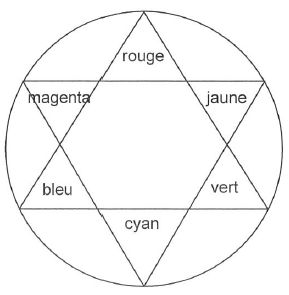
\includegraphics[width=\linewidth]{cercle}
% 	\end{center}
% \end{minipage}

\subsection{Étude cinétique de la réaction}
\subsubsection{Détermination de l'ordre partiel $p$ par rapport à l'érythrosine}

\enonce{%
	\begin{tcb}[breakable](expe)<itc>{Suivi cinétique}
		\begin{enumerate}
			\item Déconnecter le spectrophotomètre de l'ordinateur en le débranchant
			      salement (mais proprement), puis le rallumer manuellement. Fermer
			      Régression complètement.
			\item Allumer de nouveau le spectro en le rebranchant et en appuyant sur
			      \boxed{0/1}. Aller jusqu'au bout de la procédure de calibration.
			\item Eteindre le spectro en appuyant sur \boxed{0/1}. Le rallumer sous
			      contrôle de l'ordinateur comme vu précédemment. Et choisir cette fois
			      \textbf{suivi cinétique}.
			\item Indiquer la valeur de $\lambda_{\max}$ pour déterminer la longueur
			      d'onde à laquelle vous allez étudier l'évolution de l'intensité
			      lumineuse.
			\item Faire le zéro avec une cuve remplie d'eau distillée en cliquant sur
			      «~Z~».
			\item Choisir ensuite 80 points, $\delta t=\SI{4}{s}$, pour obtenir une durée
			      d'expérience de 5 min environ. Valider. Puis refaire le blanc avec la
			      cuve d'eau distillée en cliquant sur \texttt{mettre le solvant avec la
				      solution puis cliquer ici}.
			      % \begin{tcb}[cnt, bld](impo){}
			      %  La suite de la manipulation doit être effectuée rapidement pour
			      %  obtenir les premiers points, car dès le mélange entre l'érythrosine et
			      %  l'eau de Javel, la cinétique démarre.
			      % \end{tcb}
			\item Prélever à la finnpipette~: $\SI{1,2}{mL}$ d'eau de Javel,
			      \SI{1.2}{mL} d'eau distillée et $\SI{1,2}{mL}$ d'érythrosine que vous
			      déposerez successivement dans une cuve. Recouvrir de \textit{Parafilm}
			      puis mélanger \textbf{rapidement}. Déposer cette dernière dans le spectro
			      (dans le bon sens~!) et lancer l'acquisition en cliquant sur
			      \texttt{mettre la cuve avec la solution puis cliquer ici}.
			\item Une fois l'acquisition terminée, transférer les données sous Regressi en
			      cliquant sur l'icône prévue à cet effet. Créer les variables calculées
			      nécessaires, puis effectuer les régressions linéaires trouvées précédemment~;
			      les superposer avec deux échelles~: une échelle à gauche pour $lnA = \ln(A)$
			      et une échelle à droite pour $invA = 1 / A$. Supprimer les zéros en ordonnées
			      (menu coordonnées).
		\end{enumerate}
	\end{tcb}
}

\QR{%
	Effectuer les régressions linéaires pour tester les hypothèses $p = 1$ et $p
		= 2$, et imprimer les courbes. Conclure sur la valeur de $p$.
}{%
	On trouve que la régression la plus fidèle aux données est celle de $\ln A =
		f(t)$~: on en conclu que $\boxed{p=1}$.
	\begin{tcb}(rema){Remarque~: fin de cinétique}
		Quand la cinétique est terminée, la vitesse n'évolue plus. Dans ce cas, on
		peut obtenir des régressions biaisées. Il faut parfois sélectionner les
		données sur lesquelles ont fait la régression pour avoir une meilleure
		estimation du coefficient directeur.
	\end{tcb}
}
\QR{%
	Déterminer la constante apparente de vitesse de la réaction $k\ind{app,1}$ et
	le temps de demi-réaction $\tau_{1/2}$.
}{%
	Le coefficient directeur est l'opposé de la constante apparente, soit
	\[
		\xul{k\ind{app,1} = \SI{5.3e-3}{s^{-1}}}
	\]
	Et on obtient le temps de demi-réaction avec
	\[
		\boxed{t_{1/2} = \frac{\ln 2}{k\ind{app}}}
		\Lra
		\xul{t_{1/2} = \SI{131}{s}}
	\]
}

\subsubsection{Détermination de l'ordre partiel $q$ par rapport aux ions hydroxydes}

\enonce{%
	\begin{tcb}[breakable](expe)<itc>{Suivi cinétique}
		\begin{enumerate}
			\item Recommencer une nouvelle acquisition en prélevant~: $\SI{0,6}{mL}$ d'eau
			      de Javel, $\SI{1.8}{mL}$ d'eau distillée et $\SI{1,2}{mL}$ d'érythrosine. On
			      a ainsi divisé par 2 la concentration initiale des ions hypochlorites et
			      maintenue constante celle de l'érythrosine.
			\item Une fois l'acquisition terminée, transférer les données sous Regressi en
			      cliquant sur l'icône prévue à cet effet.
		\end{enumerate}
	\end{tcb}
}

\QR{%
	Vérifier l'ordre $p$ que vous avez obtenu précédemment.
}{%
	On trouve toujours une droite en traçant $\ln A = f(t)$, ce qui confirme
	l'ordre partiel 1 sur $[\ce{E}]$.
}

\QR{%
	Déterminer expérimentalement la nouvelle constante apparente de
	vitesse de la réaction, notée $k\ind{app,2}$.
}{%
	\[
		\xul{k\ind{app,2} = \SI{2.6e-3}{s^{-1}}}
	\]
}

\QR{%
	En déduire l'ordre partiel $q$ par rapport à $\ce{ClO^-}$~; l'arrondir à sa
	valeur entière la plus proche.
}{%
	On calcule avec
	\[
		\boxed{q = \frac{\ln\left(\frac{k\ind{app,1}}{k\ind{app,2}}\right)}{\ln(2)}}
		\Ra
		\xul{q = \num{1.03} \approx 1}
	\]
}

\enonce{%
	\begin{tcb}(rema){}
		Ne pas oublier d'imprimer les courbes obtenues, seuls repères pour
		l'examinataire. Vous prendrez soin de n'imprimer que les courbes et d'utiliser
		une impression noir et blanc.
	\end{tcb}
}

\section{Conclure}

\QR{%
	Quels sont les ordres partiels expérimentaux~?
}{%
	\[
		p = 1 = q
	\]
}

\QR{%
	Quel est l'ordre global de cette réaction~?
}{%
	\[
		m = p+q = 2
	\]
}

\QR{%
	Cette réaction suit-elle la loi de \textsc{Van't Hoff}~?
}{%
	Oui, car les ordres partiels sont égaux aux coefficient stœchiométriques
	arithmétiques.
}

\enonce{%
	\begin{tcb}*[cnt, bld](prop)"bomb"{Important}
		En fin de séance, nettoyez votre paillasse, débranchez le
		spectrophotomètre et ne pas oublier d'enlever la cuve à l'intérieur du
		spectrophotomètre.
	\end{tcb}
}

% \begin{programme}{}
% 
% \vspace{1cm}
% \begin{itemize}
% \item Établir une loi de vitesse à  partir du suivi 
% temporel d'une grandeur physique. 
% \item Suivi cinétique de transformations chimiques 
% \item Suivi en continu d'une grandeur physique. 
% \item Mettre en Ïuvre une méthode de suivi temporel. 
% \item Exploiter les résultats d'un suivi temporel de 
% concentration pour déterminer les caractéristiques 
% cinétiques d'une réaction. 
% \item Proposer et mettre en Ïuvre des conditions 
% expérimentales permettant la simplification de la loi 
% de vitesse. 
% \item Pratiquer une démarche expérimentale pour 
% déterminer une concentration ou une quantité de 
% matière par spectrophotométrie UV-Visible.
% \end{itemize}
% \end{programme}

\end{document}
